% ****** Start of file apssamp.tex ******
%
%   This file is part of the APS files in the REVTeX 4.2 distribution.
%   Version 4.2a of REVTeX, December 2014
%
%   Copyright (c) 2014 The American Physical Society.
%
%   See the REVTeX 4 README file for restrictions and more information.
%
% TeX'ing this file requires that you have AMS-LaTeX 2.0 installed
% as well as the rest of the prerequisites for REVTeX 4.2
%
% See the REVTeX 4 README file
% It also requires running BibTeX. The commands are as follows:
%
%  1)  latex apssamp.tex
%  2)  bibtex apssamp
%  3)  latex apssamp.tex
%  4)  latex apssamp.tex
%
\documentclass[%
 reprint,
 amsmath,amssymb,
 aps,
]{revtex4-2}
\usepackage{graphicx}% Include figure files
\usepackage{dcolumn}% Align table columns on decimal point
\usepackage[utf8]{inputenc}
\usepackage[english]{babel}
%\usepackage{authblk} % For author and affiliation handling
\usepackage{biblatex}
\addbibresource{sorsamp.bib}
\usepackage{bm}% bold math


\begin{document}

\preprint{APS/123-QED}

\title{Rise of an alternative majority against mass media in an opinion formation model}% Force line breaks with \\

\author{Jordan Zambrano$^{1}$}
\affiliation{$^1$School of Physical Sciences and Nanotechnology, Yachay Tech University, Urcuqui, Ecuador}
\author{Mario Cosenza$^{1}$}
\affiliation{$^1$School of Physical Sciences and Nanotechnology, Yachay Tech University, Urcuqui, Ecuador}





\date{\today}% It is always \today, today,
             %  but any date may be explicitly specified

\begin{abstract}
In this work it is analyzed the behavior of a system of opinion dynamics. There are considerate some important aspects in sociophysics and computational sociology, like homophilia and the interaction as a factor of a threshold. Also there is added the component of mass media, expressed as a external field, that affect all the individuals in a system. For this work is considered a global network in which all individuals of the system are connected to all the others. There is explored the space of parameters, considering three parameters: threshold of interaction $\mu$, level of interaction with mass media influence $\beta$, and the massage this mass media will reproduce $\lambda$, there are presented some phase diagrams that show the behavior of system along these spaces.

\end{abstract}

%\keywords{Suggested keywords}%Use showkeys class option if keyword
                              %display desired
\maketitle

%\tableofcontents

\section{Introduction }


% Talk about of the type of opinions in detail, look for bibliograpy
% talk about studies around mass media effects

% talk about the possible results of simulations: concesus, diversity and the emergence of new mayority state 



\section{Methodology}
For this work it is considered a global network, in which all nodes are connected and interact with all the other nodes, or at least has the possibility to do in this way, because there are considered some threshold conditions. Also for this system there are taken discrete opinion state, this is there would be $p$ available opinion options, in that sense all this work will be done with the fixed value $p = 100$. As this work deals with ranked opinions our space of possible states is $0-99$. In a similar way of a punctuation system of any product or film, in which one can offer a grade or qualification in a discrete range of graduated options.

For developing algorithm of simulation there are considered some important aspects, like the selection of parameters it would be configured to change and with which are possible to change the properties and performance of the system in general. Following the development in the previous section, there are considered parameters like $\beta$ that encode the intensity of the external field (mass media) in a way of probability of an specific node to interact with the external field. Notice also that the difference $1 - \beta$ is the probability of the node to interact with any other member of the network and not with the mass media.



There is also defined the fixed state of the external field $M$, that encode the opinion state spread by mass media. This is used to define a distance value between any node that tries to interact with external field. Having this difference is compared with the value of tolerance $\mu$, a way of threshold that define the maximum distance in the opinion space that make it possible for two nodes or the node-field to interact. Notice that the value $\mu$ is the same for both interactions, as it can be seen in Figure \ref{fig:flux_diagram_1}.
\begin{figure}
    \centering
    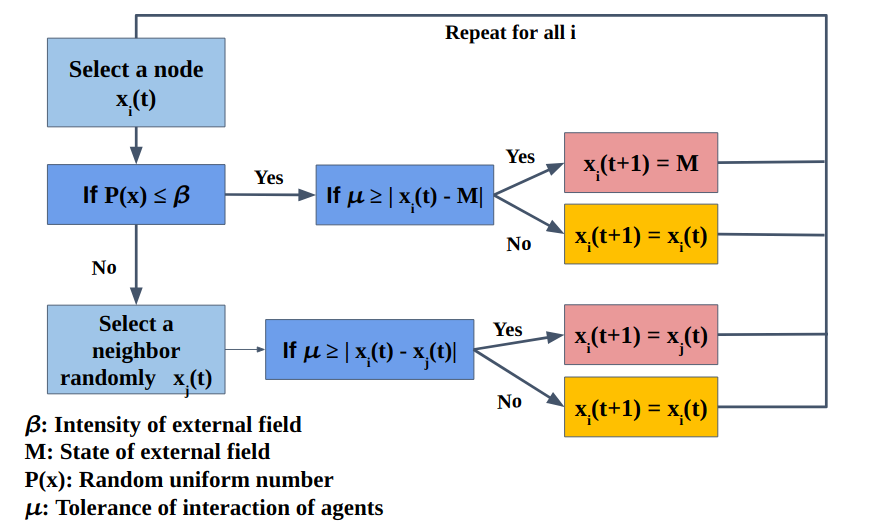
\includegraphics[width=1\linewidth]{images/Screenshot from 2024-08-21 11-15-28.png}
    \caption{Flux diagram of Algorithm used for the simulation of the system.}
    \label{fig:flux_diagram_1}
\end{figure}

In this point the way this system made nodes interact, with other nodes or with external field, is by copying the state of the other. This is, if the condition of threshold if fulfil then the node will copy the state the neighbour or the state of mass media, in the correspondent case. The process starts with a random initial position, with random value following a uniform distribution, and is executed iteratively until is a stationary state in all system is reached.

After this, it is defined the way of experimentation over simulations would be, for that there are defined some metrics that help to evaluate the results of simulations as well as compare the effect of different parameters evolution. For this work is used the value $S_{max}$ that will reveal the relative size of the bigger opinion group, the proportion of nodes with the specific opinion state that has more size. It is also used the value of $\sigma$ that represent the size difference between the $S_{max}$ and the opinion state in which external field is fixed. 

After this point there are conducted simulations of the systems described, considering $50$ repetitions of simulations. There are presented some phase diagrams that relate the behavior of the systems under specific conditions. This work explores the effect of different values of contains expressed throughout parameters, under some specific domains. For example the parameter $\beta$ because of being a probability is marked between $0$, and $1$, and the case of the tolerance $\mu$, goes from $0$ to the size of the opinion state space. In the same way the value of $M$, that is fixed in the same space that the available option states. 


\section{Results and Discussion}


For the presentation of results, there are considered some cases to illustrate the state of art and also to understand the behavior of the system with the less influences, this is the system that considers a null influence of external field, when $\beta =0$, and all the interactions of nodes is with other nodes. This case is presented in Figure. \ref{fig:sigma_prop_vs_tolerance_i0}. Each point represents a fixed state in the parameters space, it means a set of realizations of the system for each dot of the plot. And what can be seen is the almost linear and direct proportionality of the $S_{max}$ metric, with respect the value of the threshold fixed, for small values of $\mu/p$. But as this value increases to $1$ the profile get constrained and the shape of the profile closes to a square root relation.

\begin{figure}
    \centering
    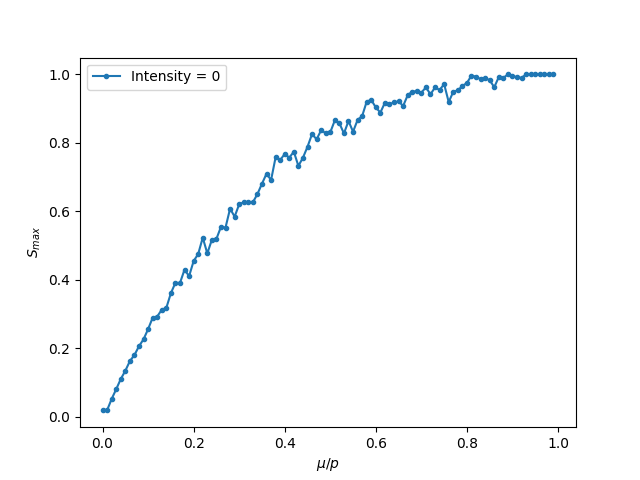
\includegraphics[scale = 0.45]{images/profile_intensity0.png}
    \caption{Profile of $S_{max}$ against normalized tolerance $\mu/p$ for a fixed intensity of mass media $\beta =0$.}
    \label{fig:sigma_prop_vs_tolerance_i0}
\end{figure}

As we change the value of some of the parameters described, it will be found that the performance and the state of the system will show some different behaviors. For the next figure there is presented a more general plot in which are include a new parameter dimension, which is $\beta$. In Fig. \ref{fig:conbined_plot} it is shown the $\log \sigma$ relation as function of $\mu/p$ and $\beta$, as well as there are presented different plots for the message imposed by mass media, in the same range of $\mu$, the tolerance of the system.

\begin{figure*}
    \centering
    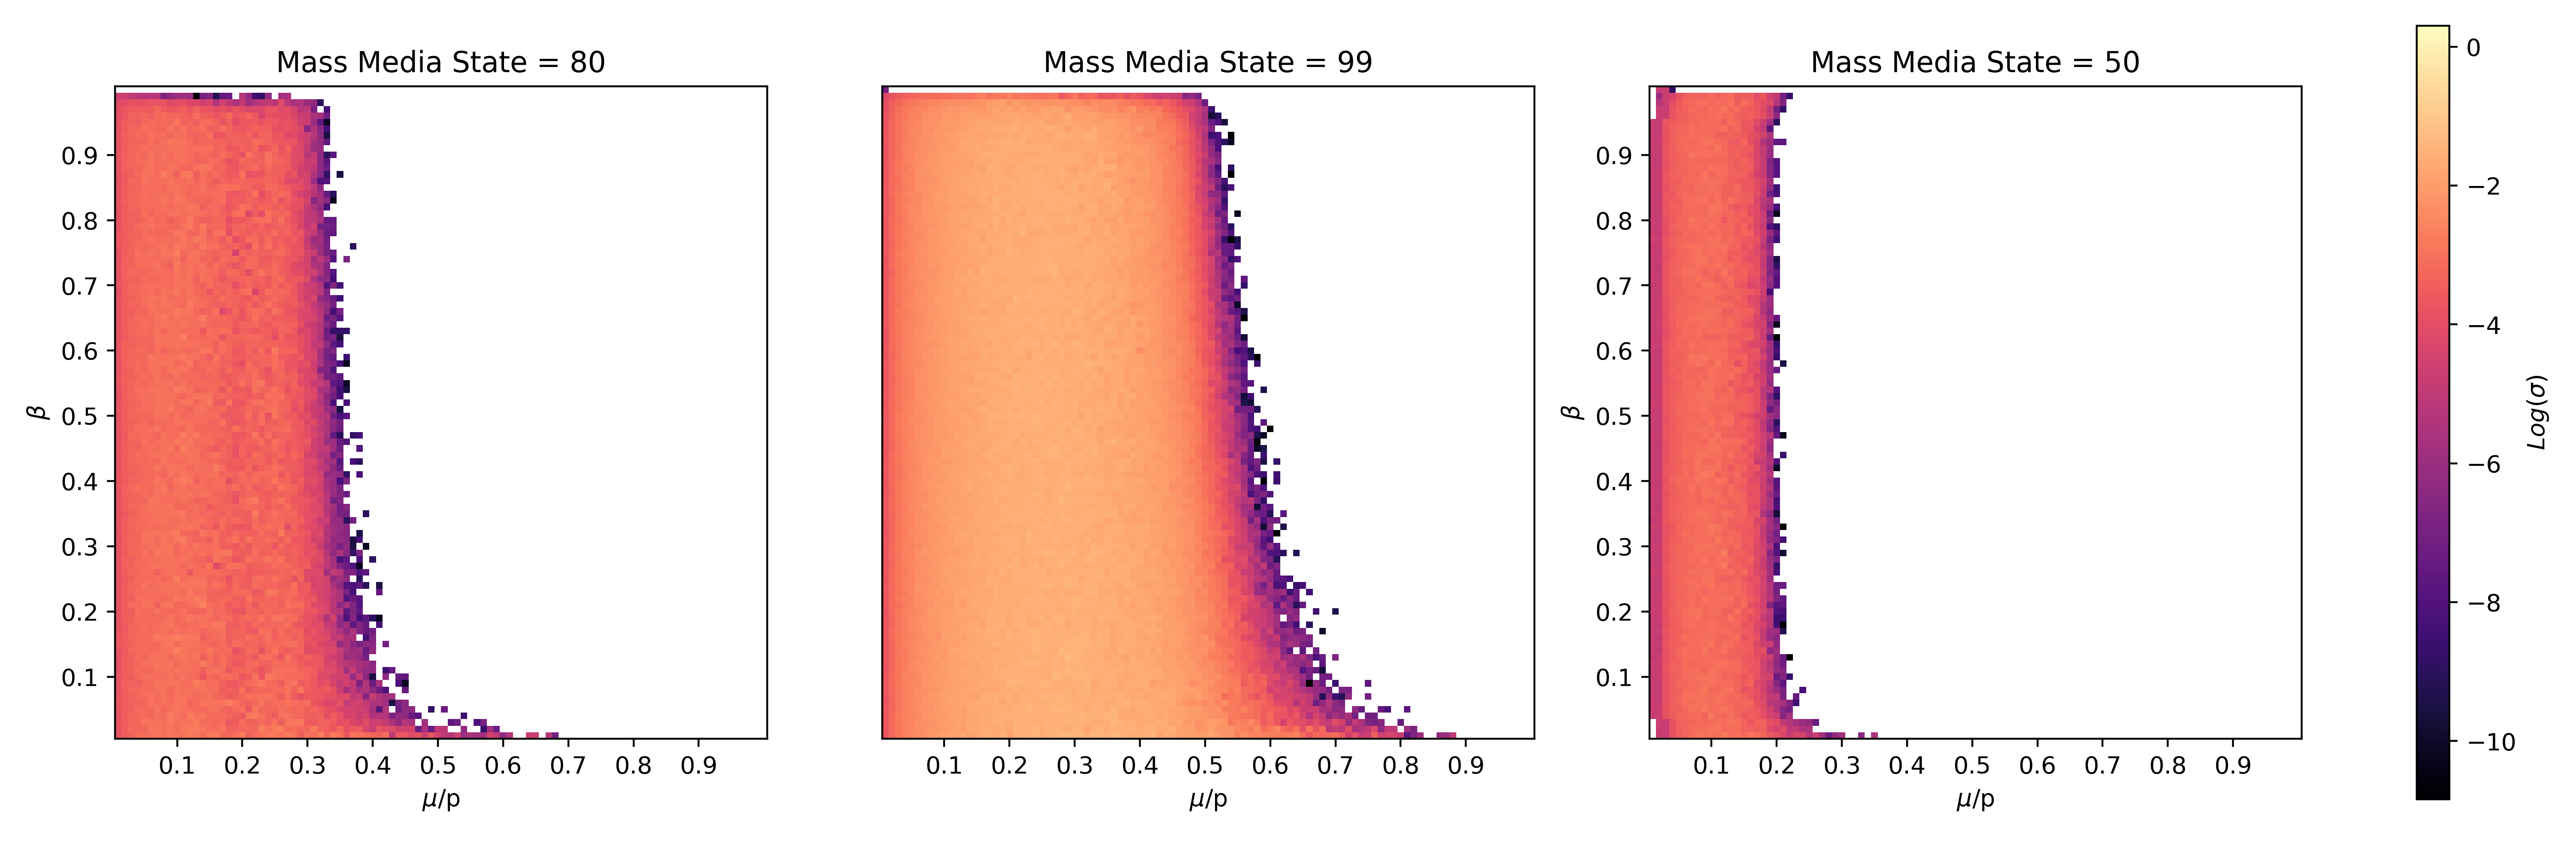
\includegraphics[scale = 0.5]{images/combinened_logplot_prop80-99-50.png}
    \caption{Heat maps of the $\log{\sigma}$ in function of parameters: $\mu/p$ and $\beta$, normalized tolerance and mass media intensity respectively. Each plot uses different values of the mass media state : $80$, $99$, $50$ respectively from left to right.}
    \label{fig:combined_plot}
\end{figure*}


\begin{figure}
    \centering
    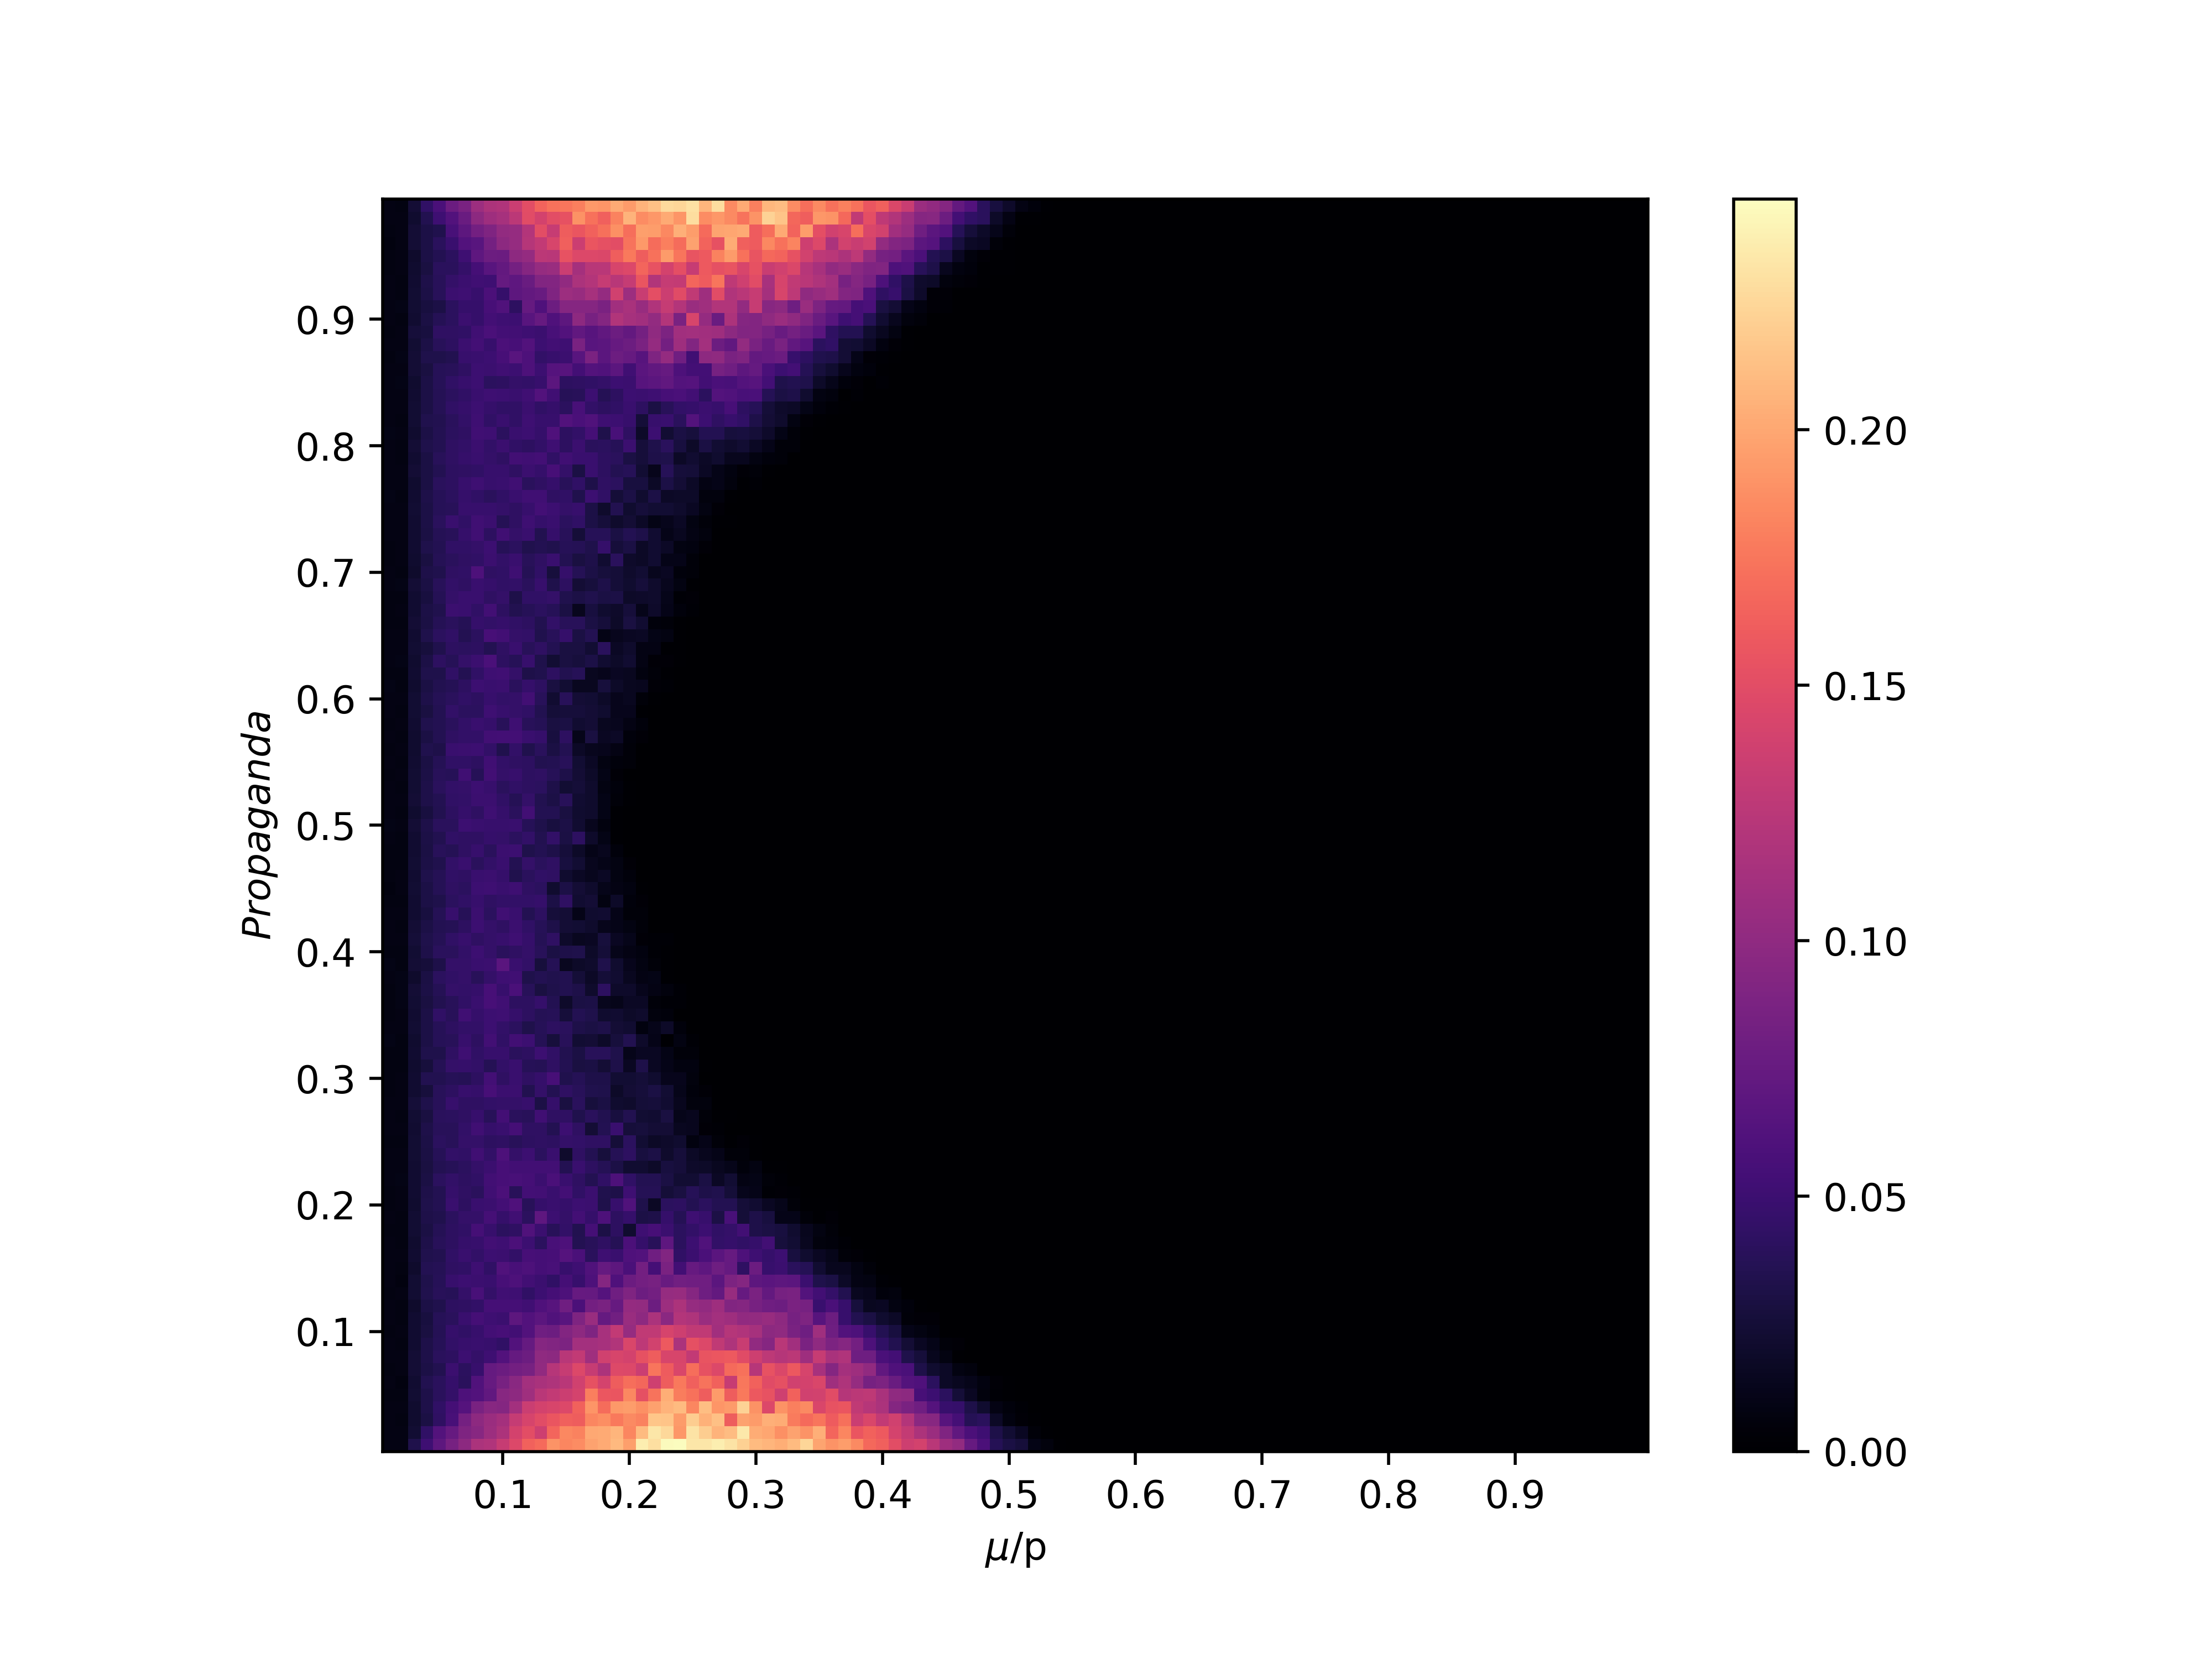
\includegraphics[scale = 0.45]{images/global_prop_vs_mu_n1000_p100_i050.png}
    \caption{Heat map of $\sigma$ in function of normalized tolerance $\mu/p$ and the mass media state for fixed value of intensity $\beta = 0.5$.}
    \label{fig:sigma_prop_vs_tolerance_i05}
\end{figure}

\begin{figure}
    \centering
    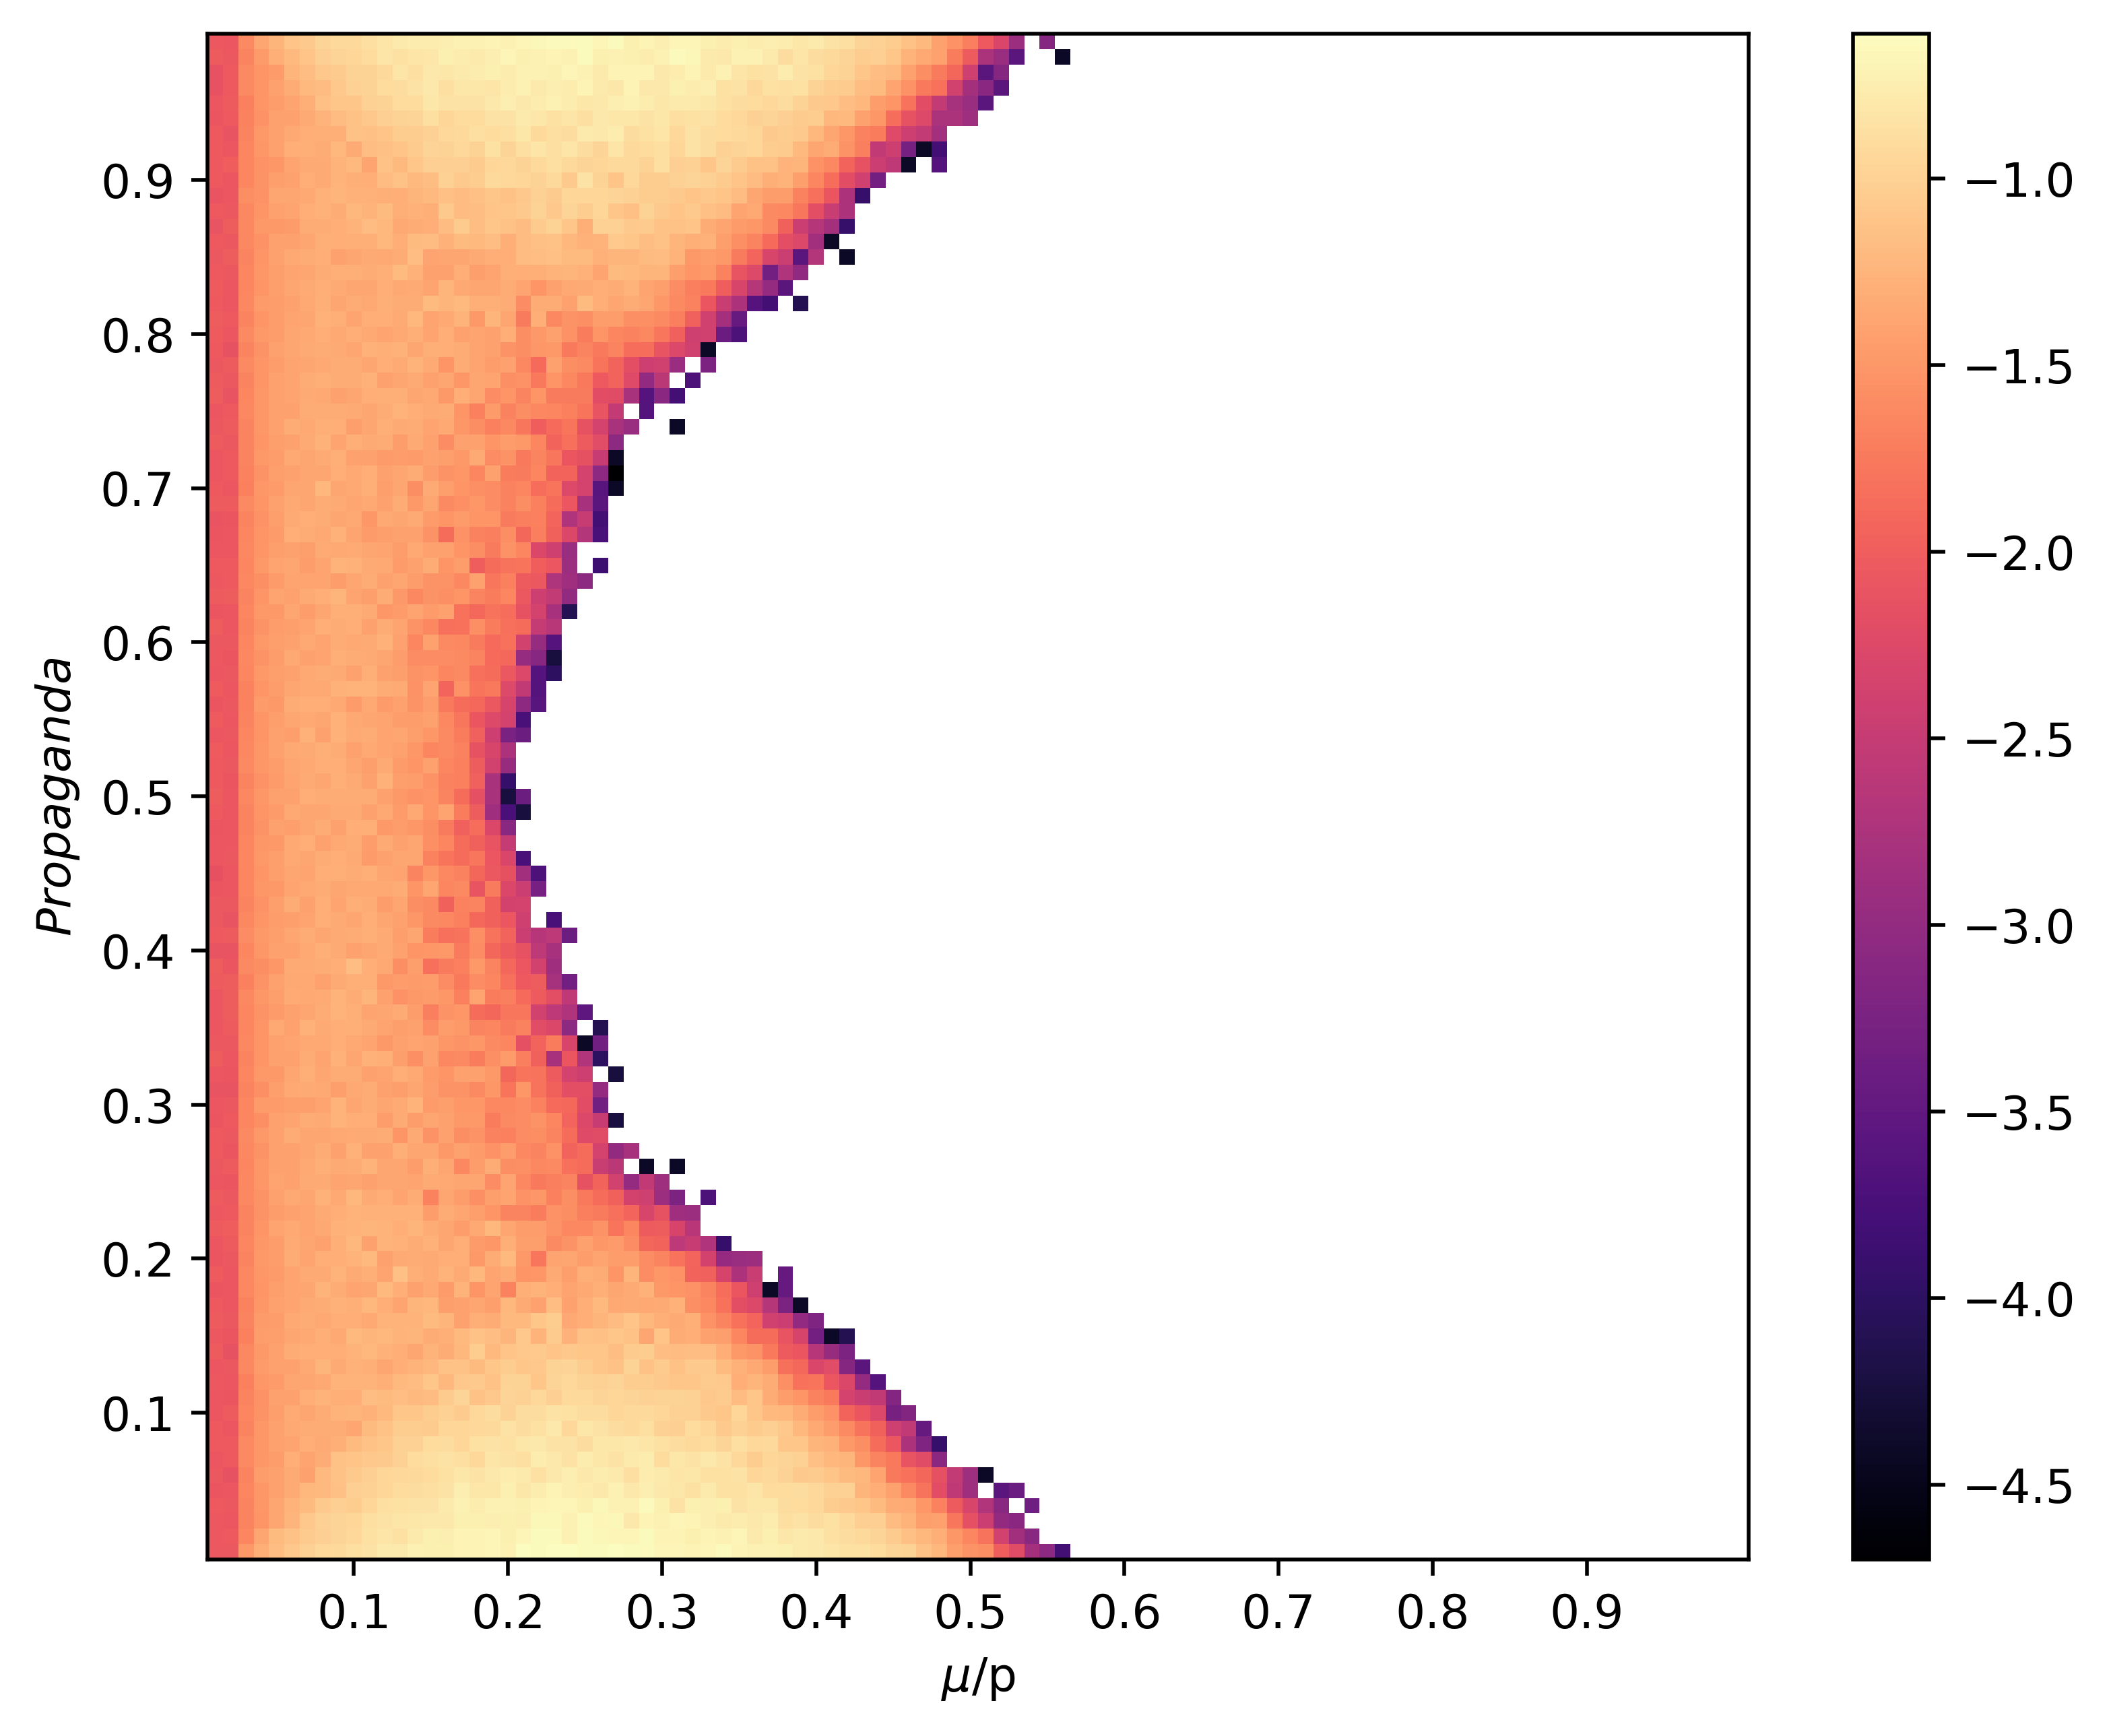
\includegraphics[scale = 0.45]{images/log_sigma_prop_vs_mu_b05.png}
    \caption{Heat map of \log($\sigma$) in function of normalized tolerance $\mu/p$ and the mass media state for fixed value of intensity $\beta = 0.5$.}
    \label{fig:logsigma_prop_vs_tolerance_i05}
\end{figure}

\begin{figure}
    \centering
    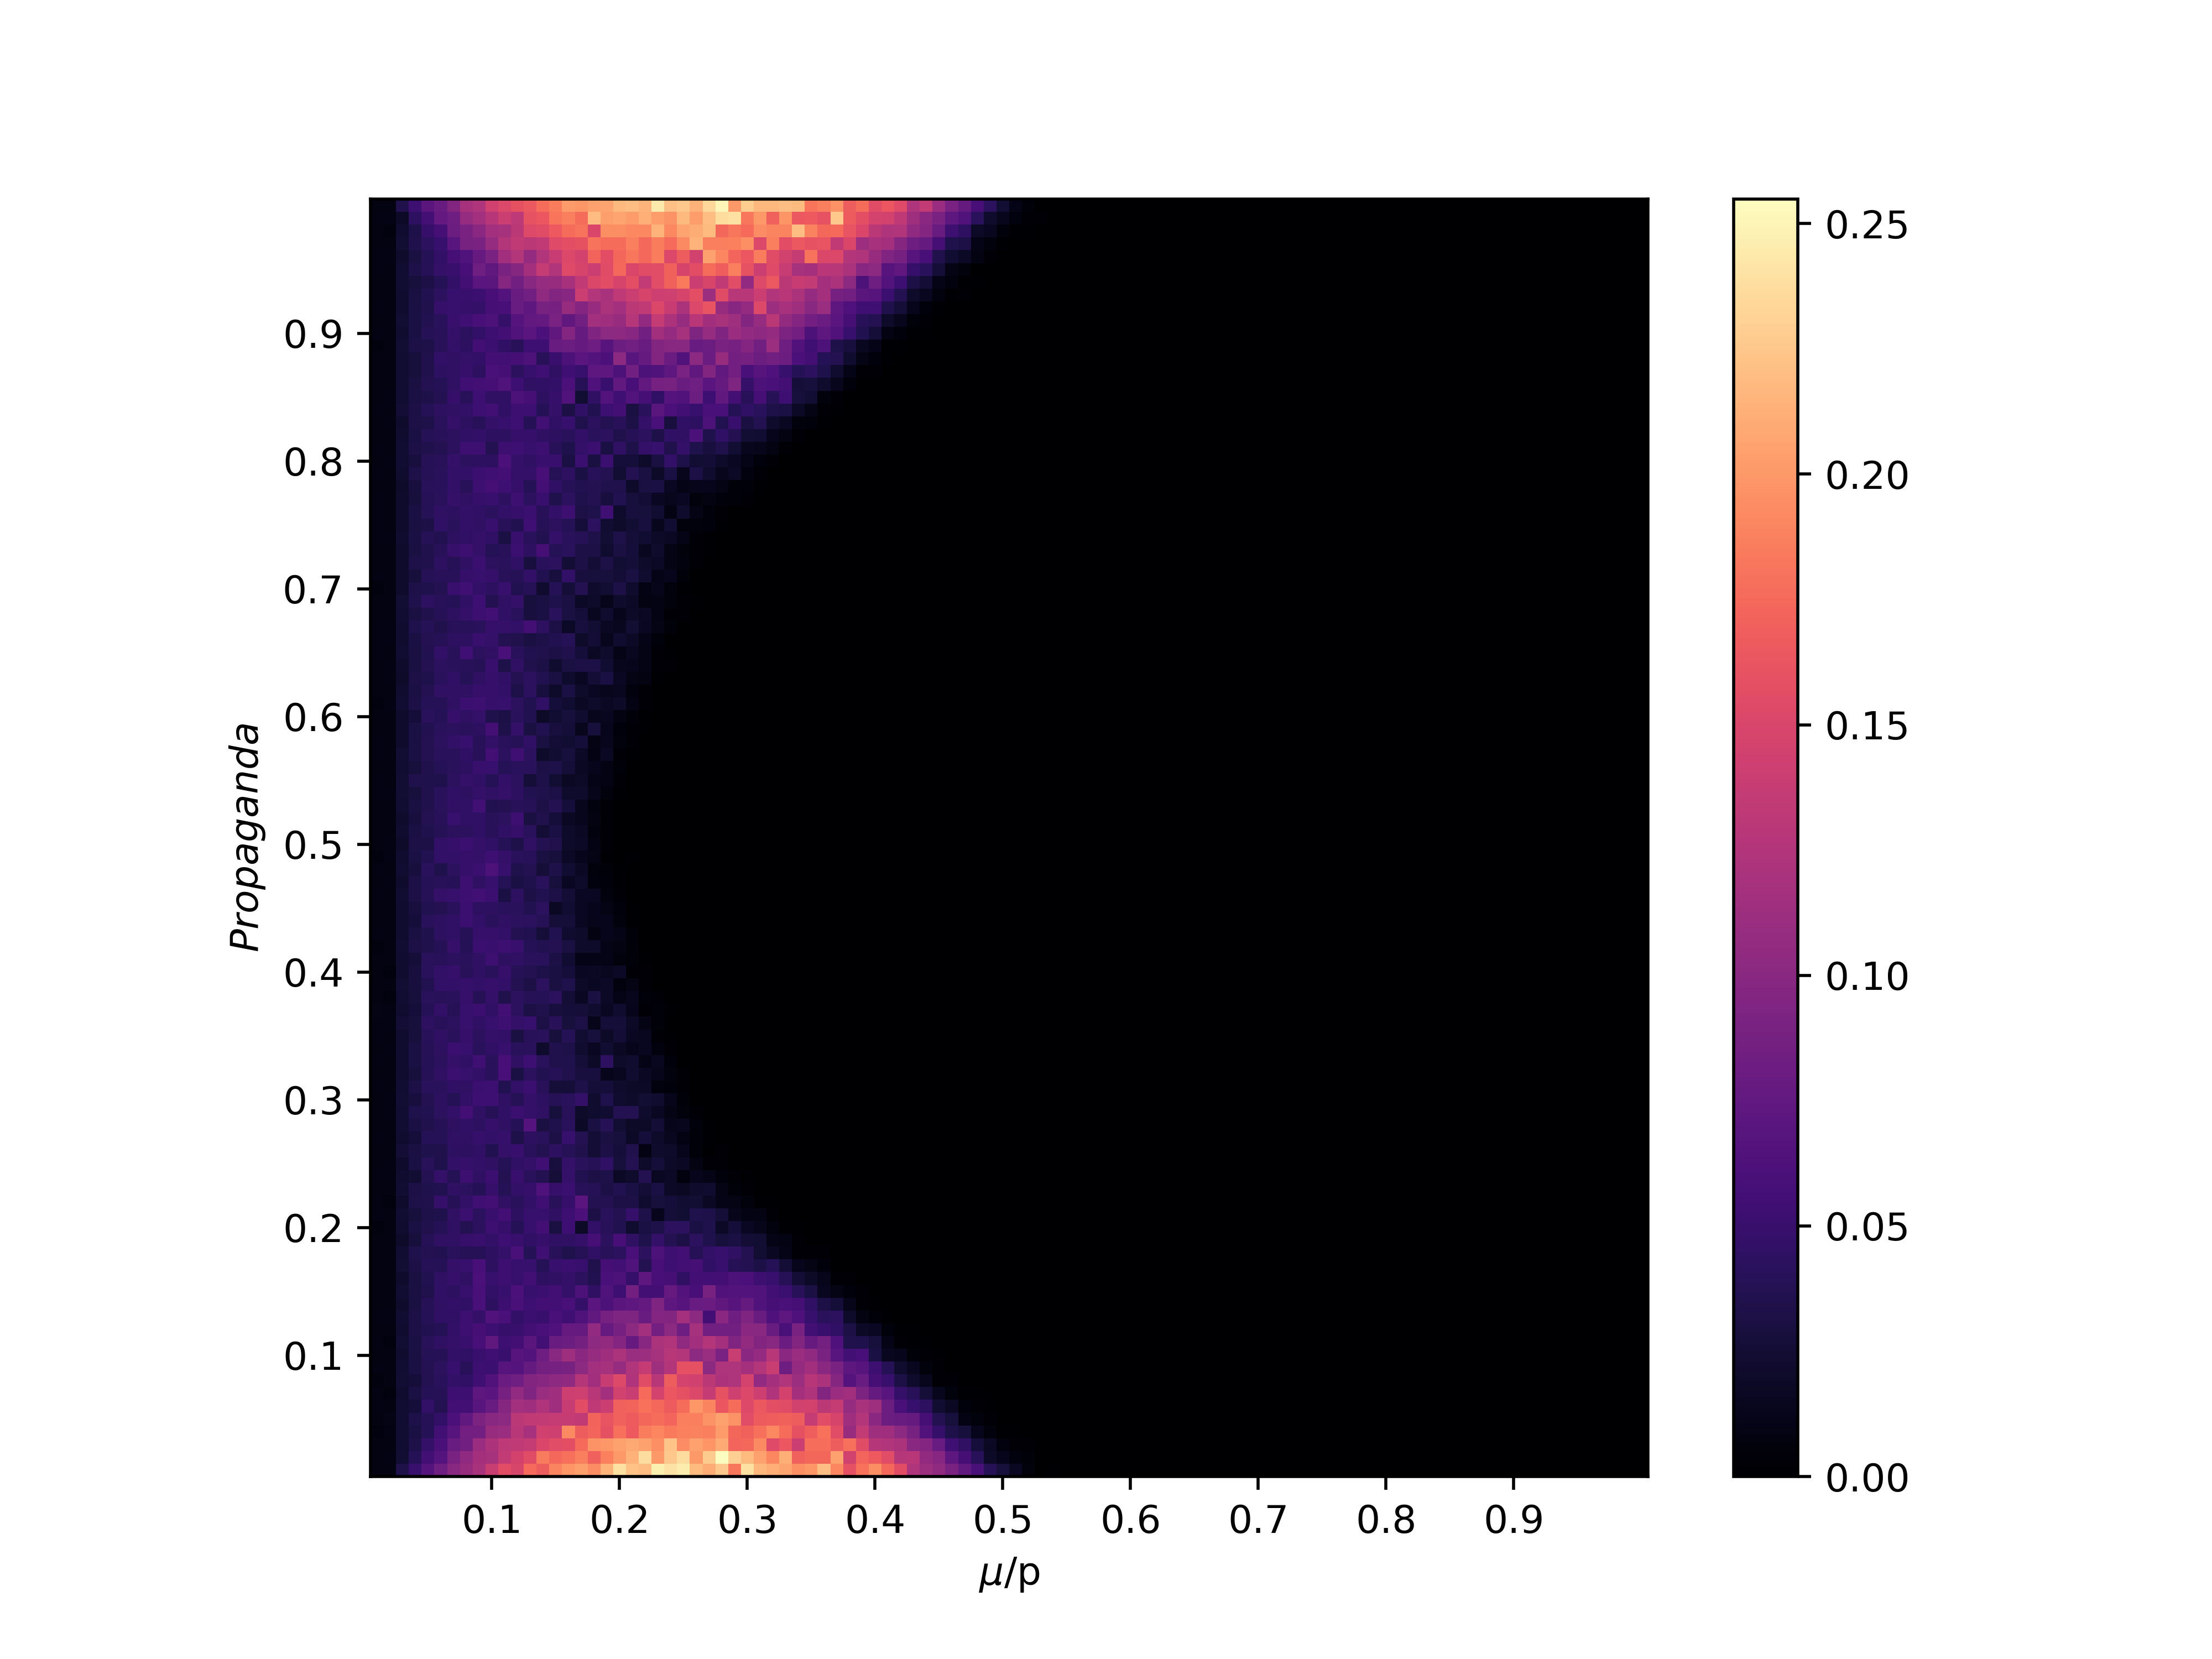
\includegraphics[scale = 0.45]{images/sigma_prop_vs_mu_b08.png}
    \caption{Heat map of $\sigma$ in function of normalized tolerance $\mu/p$ and the mass media state for fixed value of intensity $\beta = 0.8$.}
    \label{fig:sigma_prop_vs_tolerance_i08}
\end{figure}
\begin{figure}
    \centering
    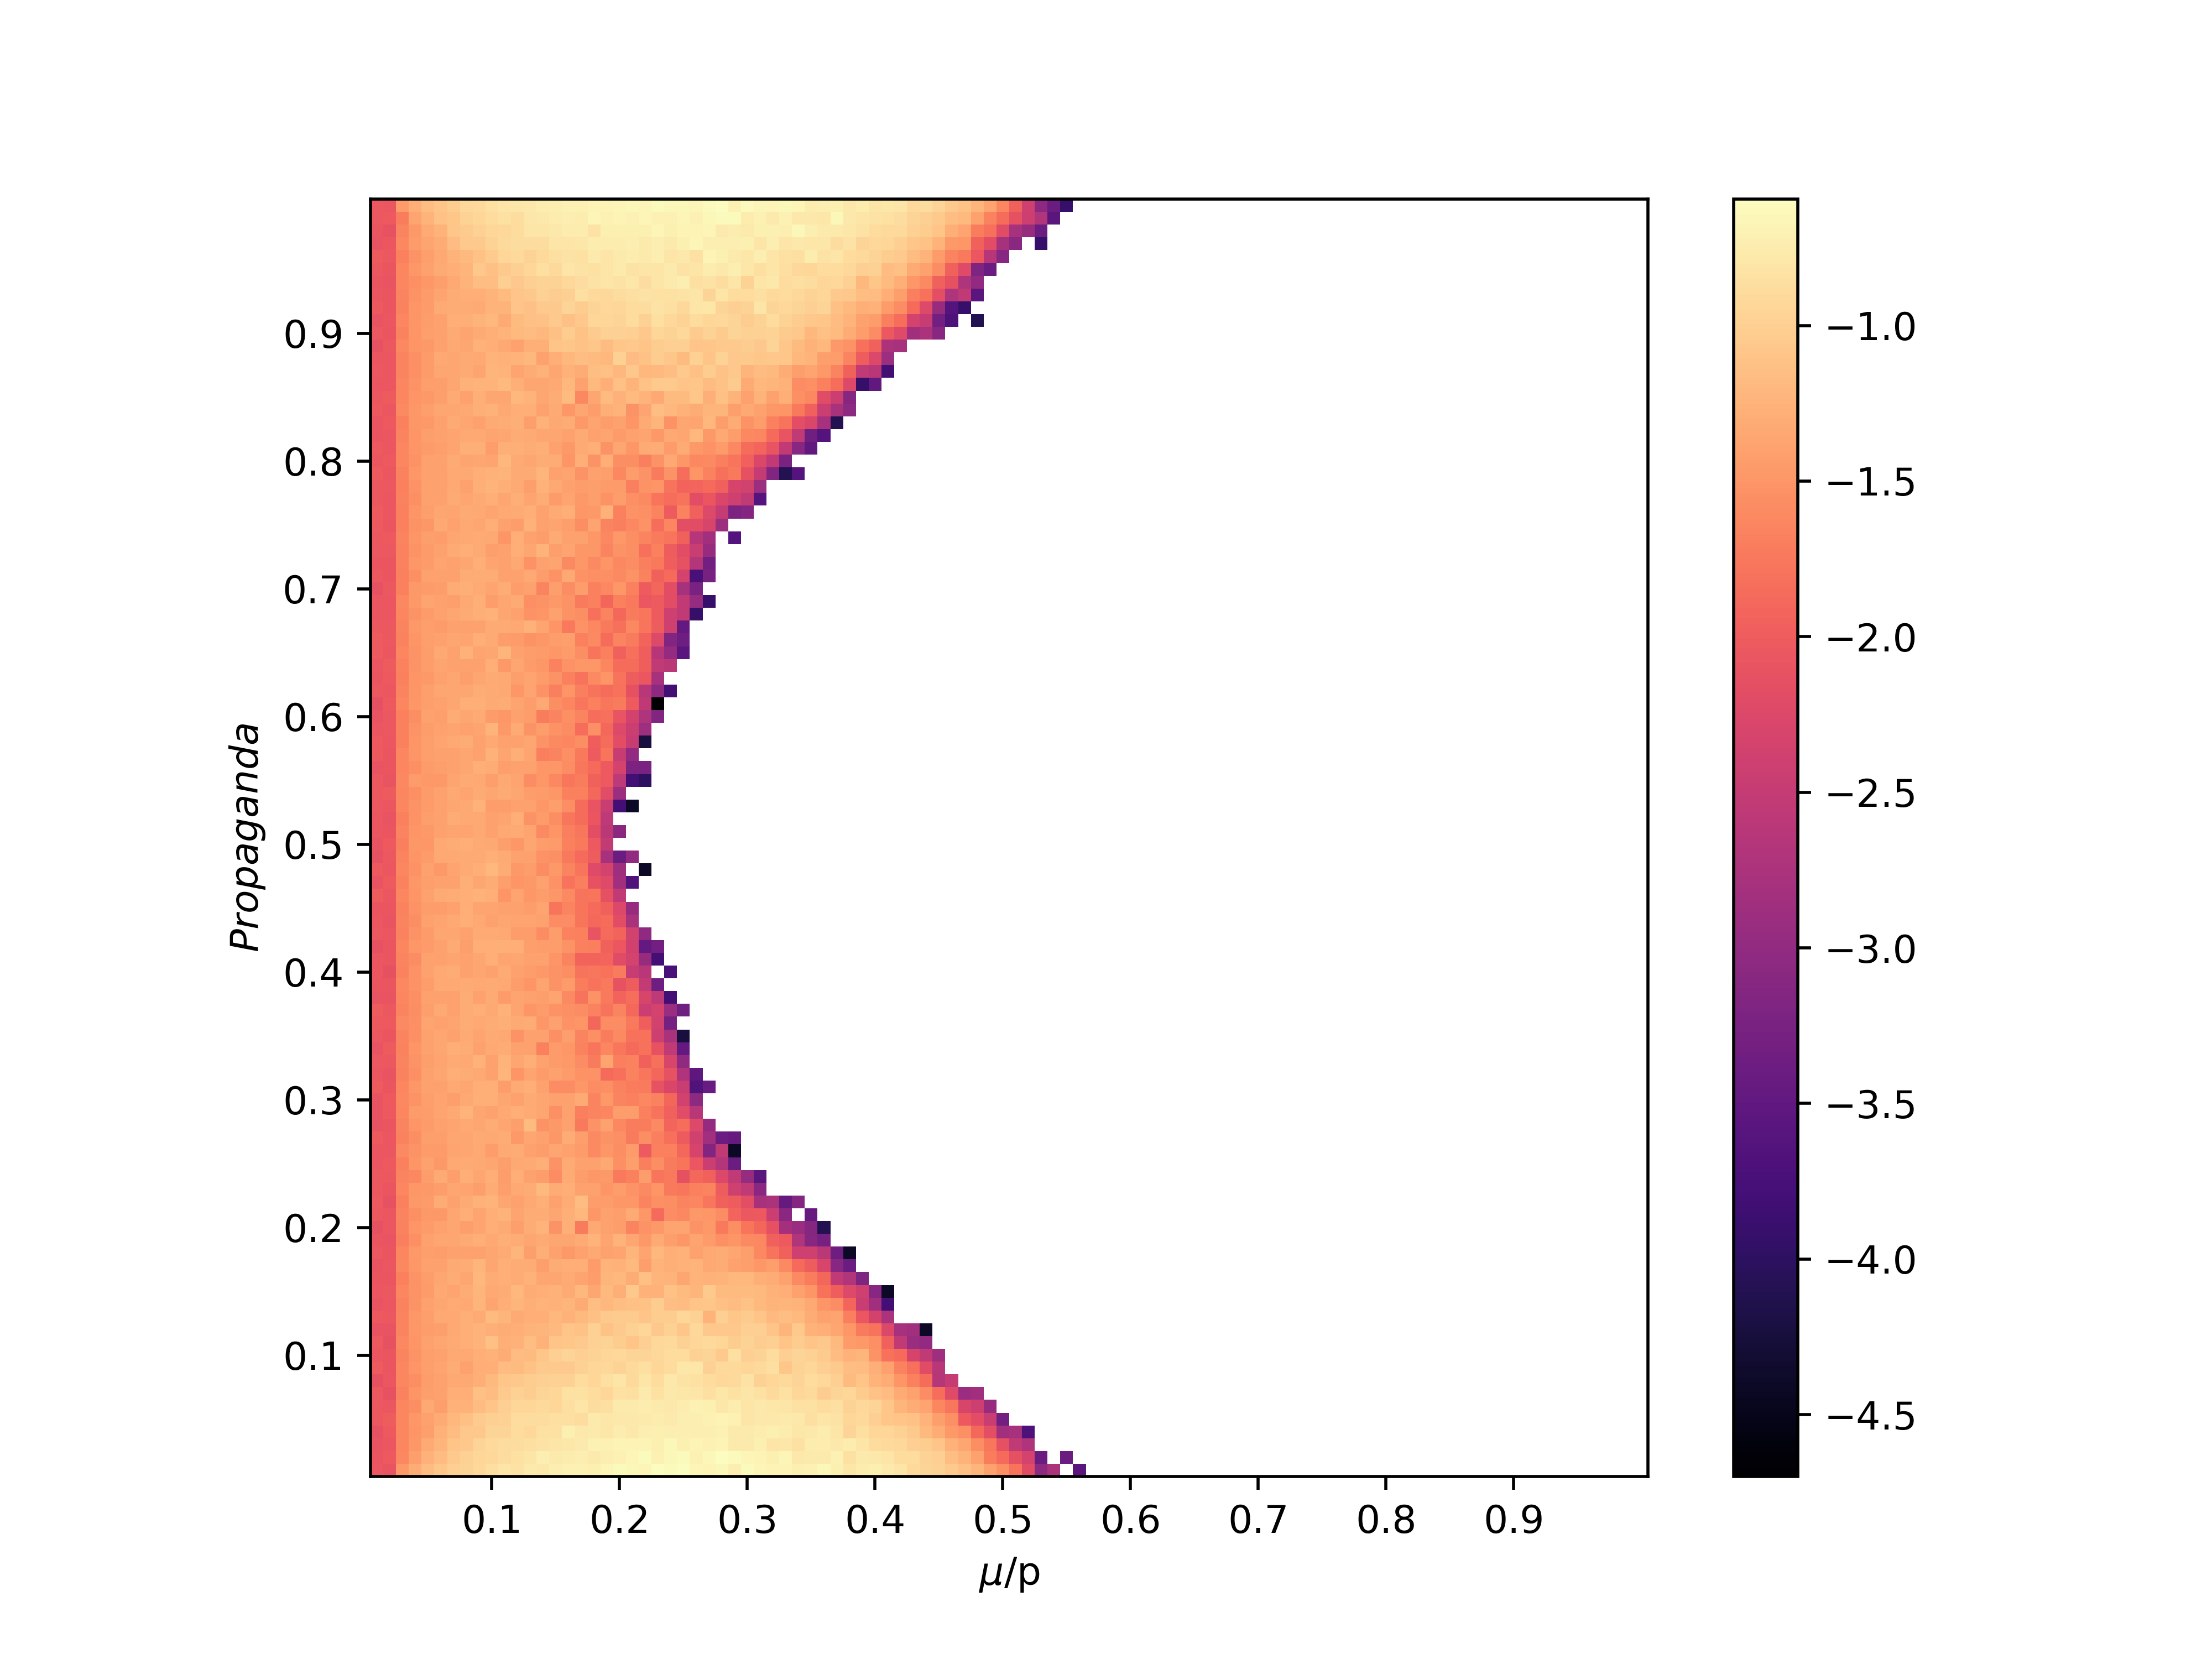
\includegraphics[scale = 0.45]{images/log_sigma_prop_vs_mu_b08.png}
    \caption{Heat map of \log($\sigma$) in function of normalized tolerance $\mu/p$ and the mass media state for fixed value of intensity $\beta = 0.8$.}
    \label{fig:logsigma_prop_vs_tolerance_i08}
\end{figure}


\begin{figure}
    \centering
    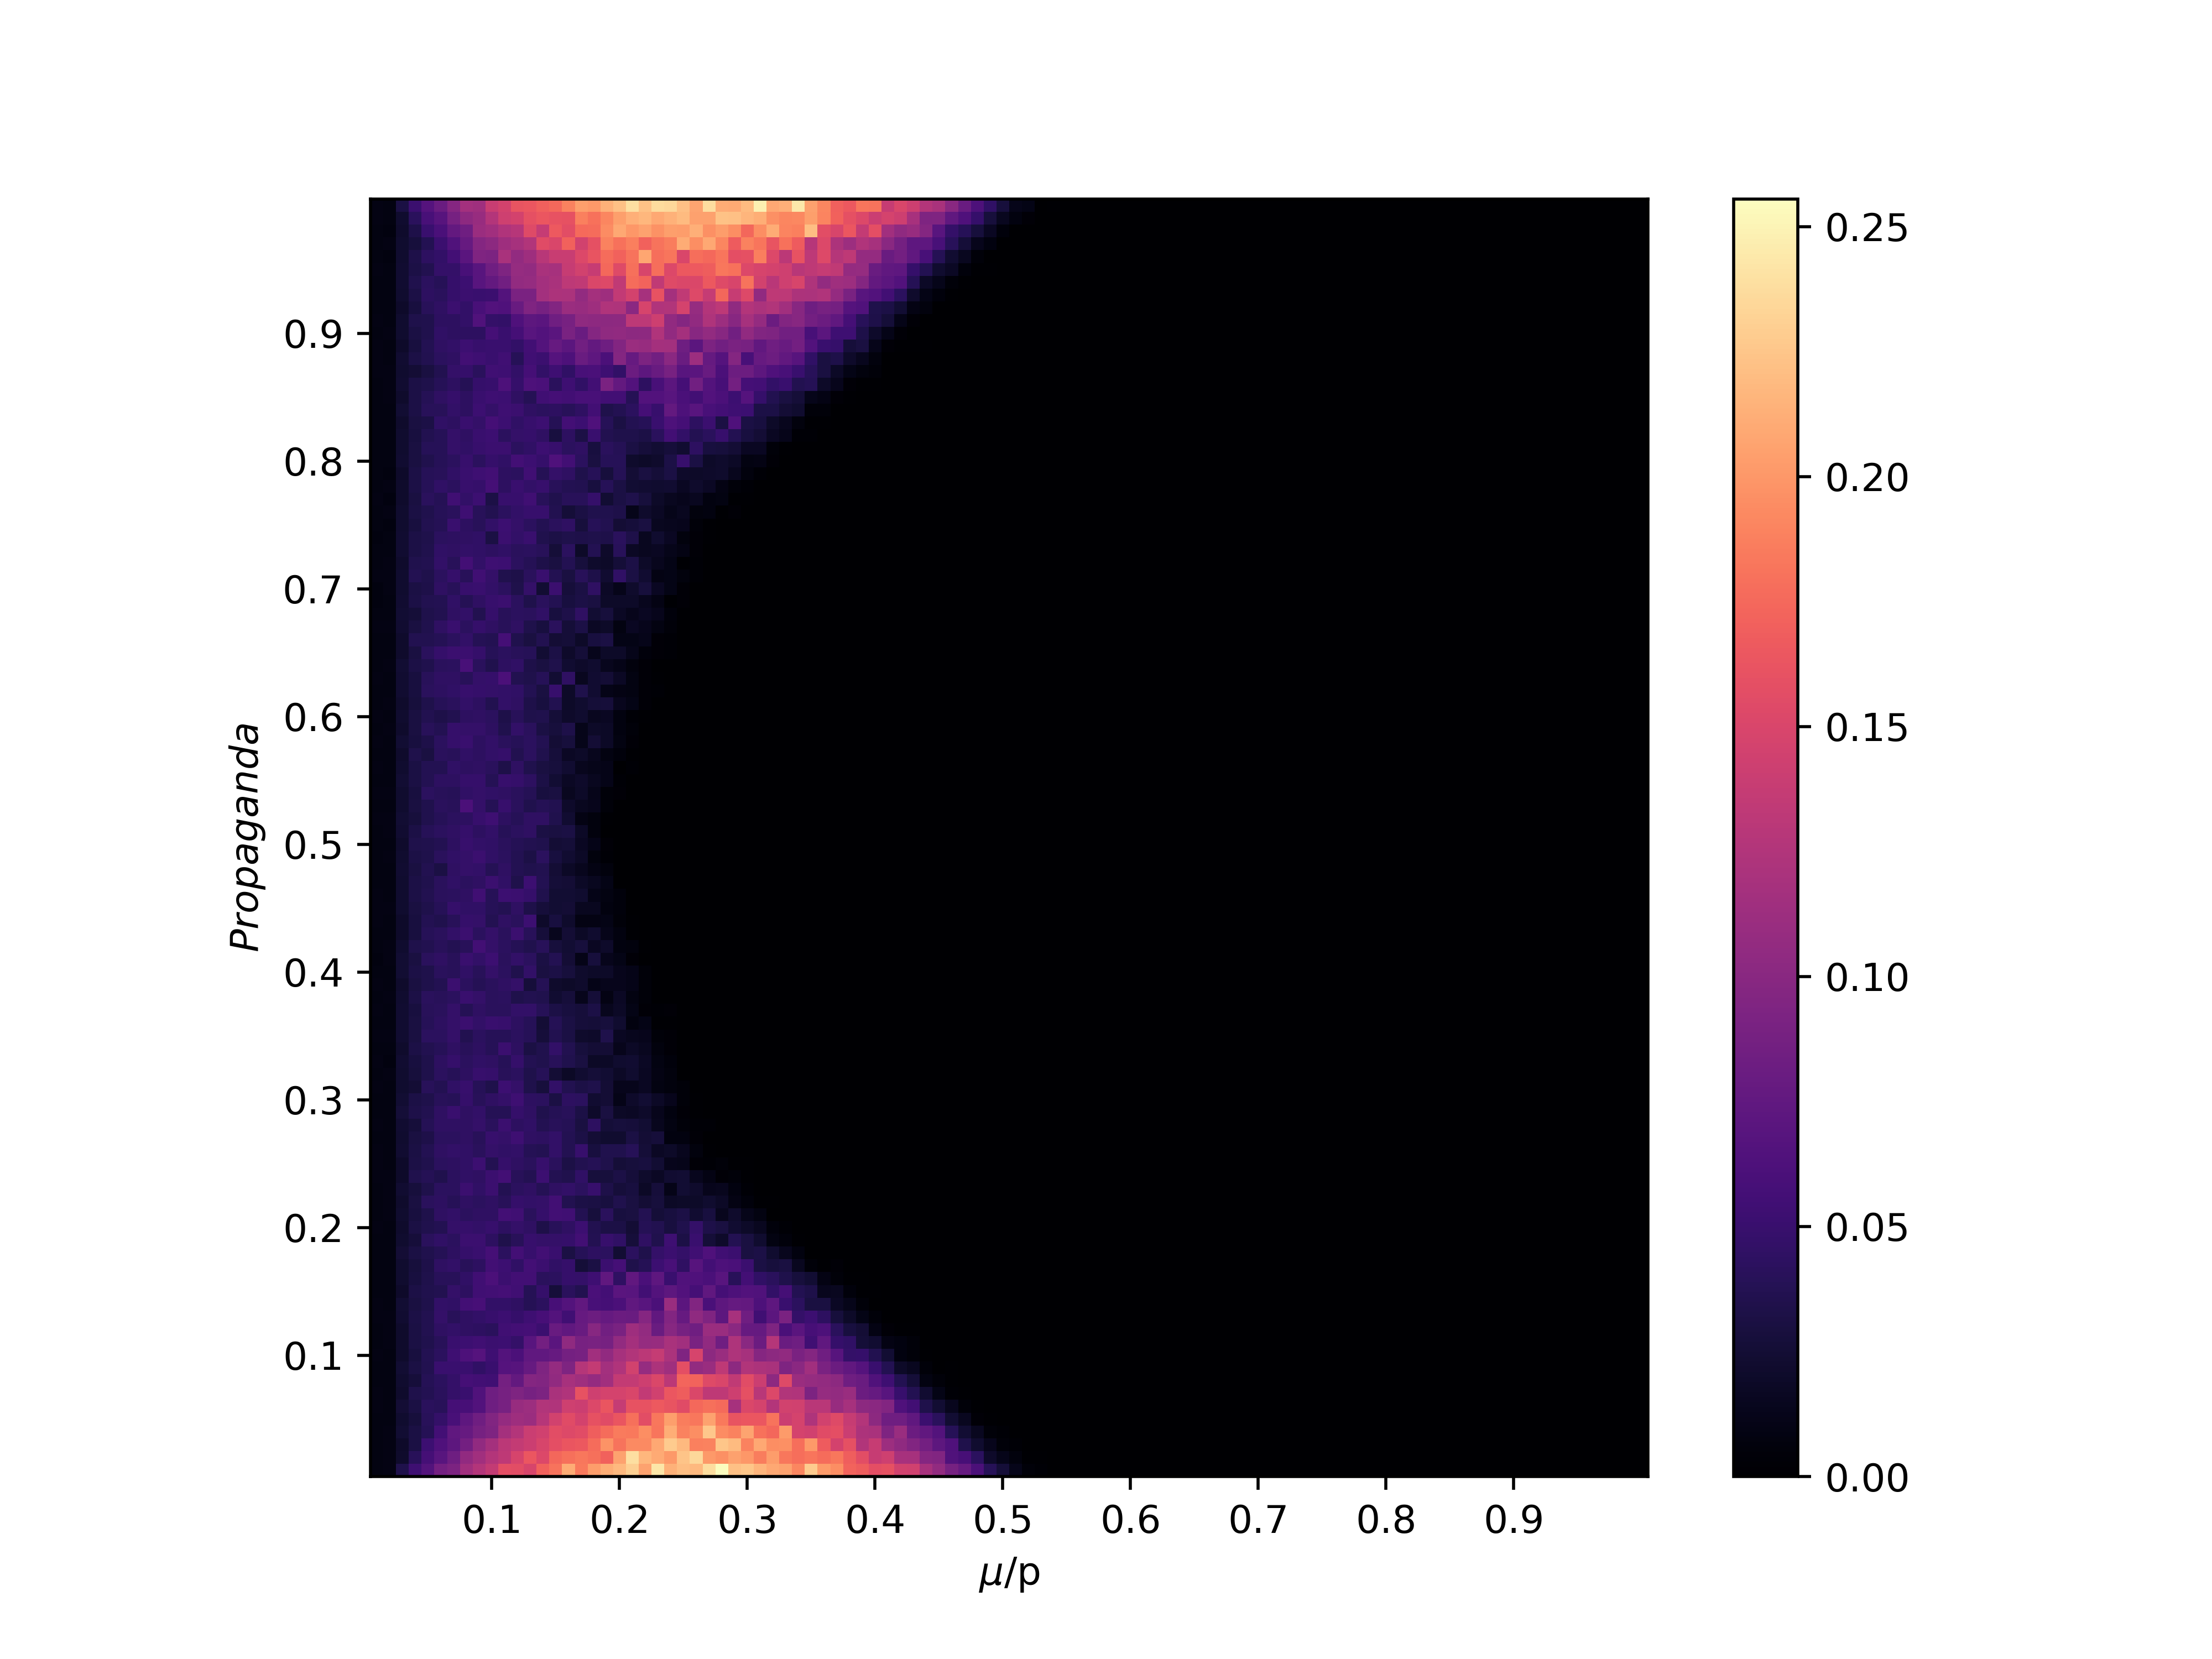
\includegraphics[scale = 0.45]{images/sigma_prop_vs_mu_n1000_p100_i09.png}
    \caption{Heat map of $\sigma$ in function of normalized tolerance $\mu/p$ and the mass media state for fixed value of intensity $\beta = 0.9$.}
    \label{fig:sigma_prop_vs_tolerance_i09}
\end{figure}
\begin{figure}
    \centering
    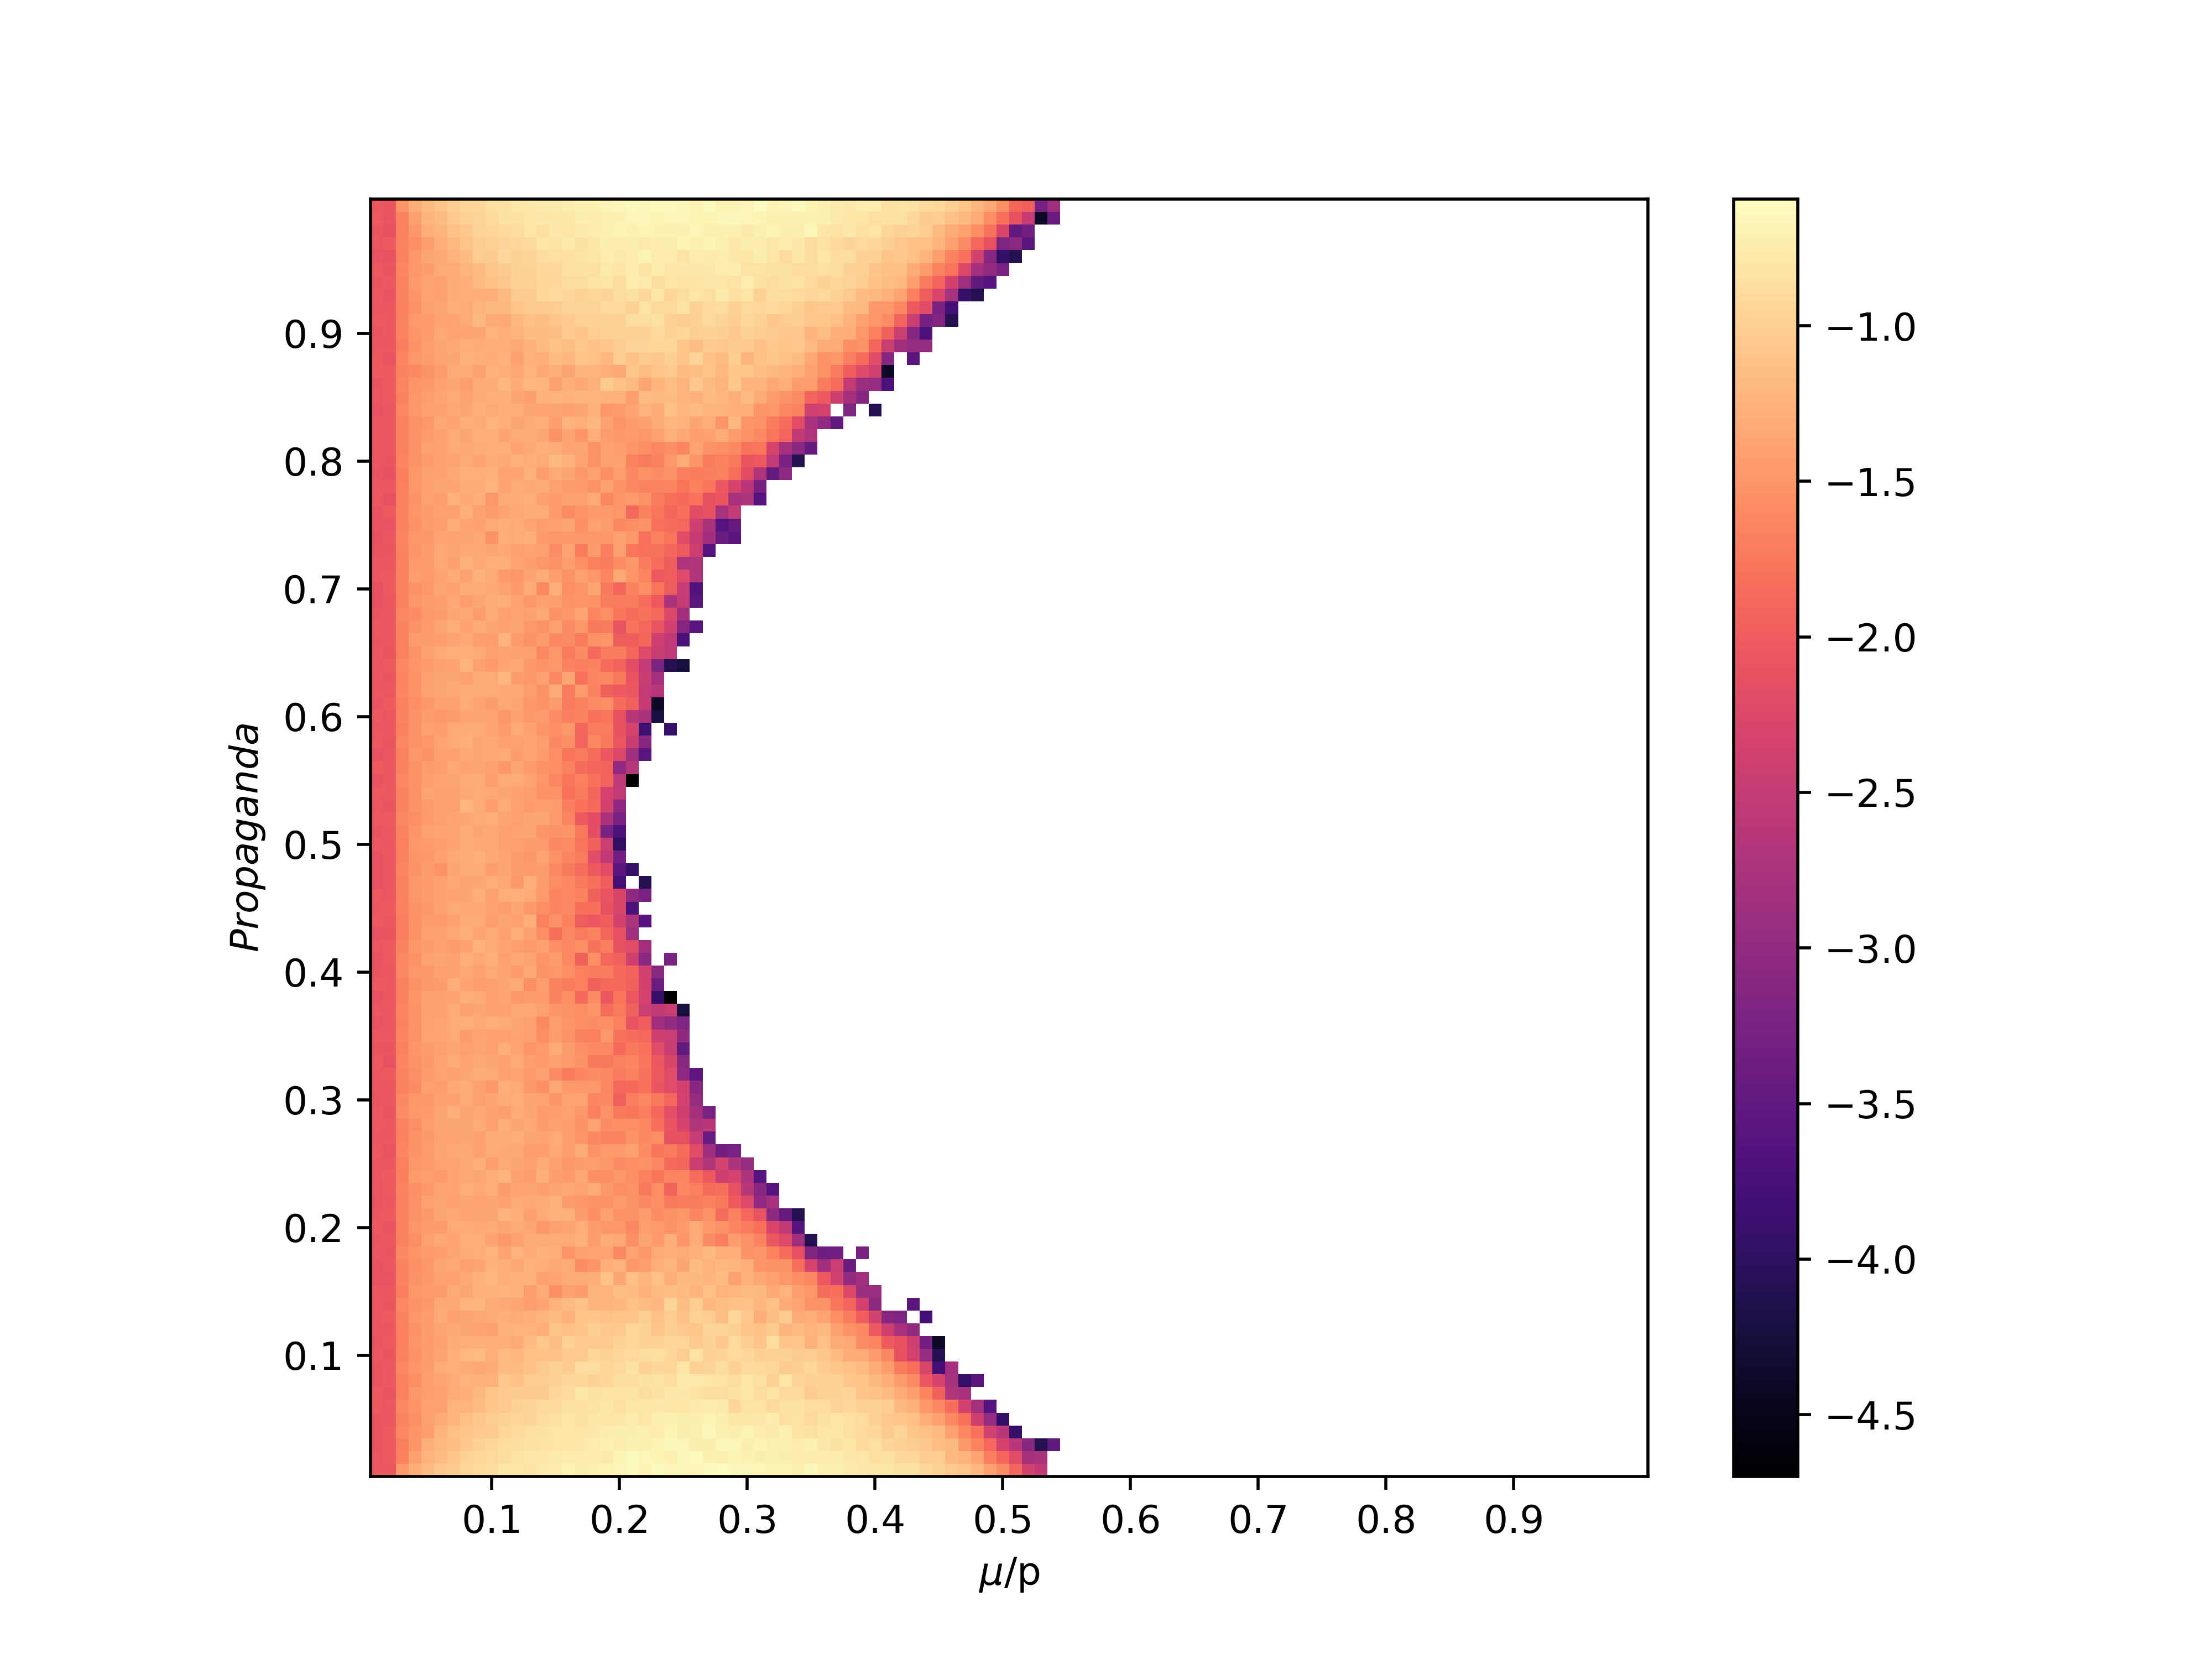
\includegraphics[scale = 0.45]{images/log_sigma_prop_vs_mu_n1000_p100_i09.png}
    \caption{Heat map of \log($\sigma$) in function of normalized tolerance $\mu/p$ and the mass media state for fixed value of intensity $\beta = 0.9$.}
    \label{fig:logsigma_prop_vs_tolerance_i09}
\end{figure}

\begin{figure}
    \centering
    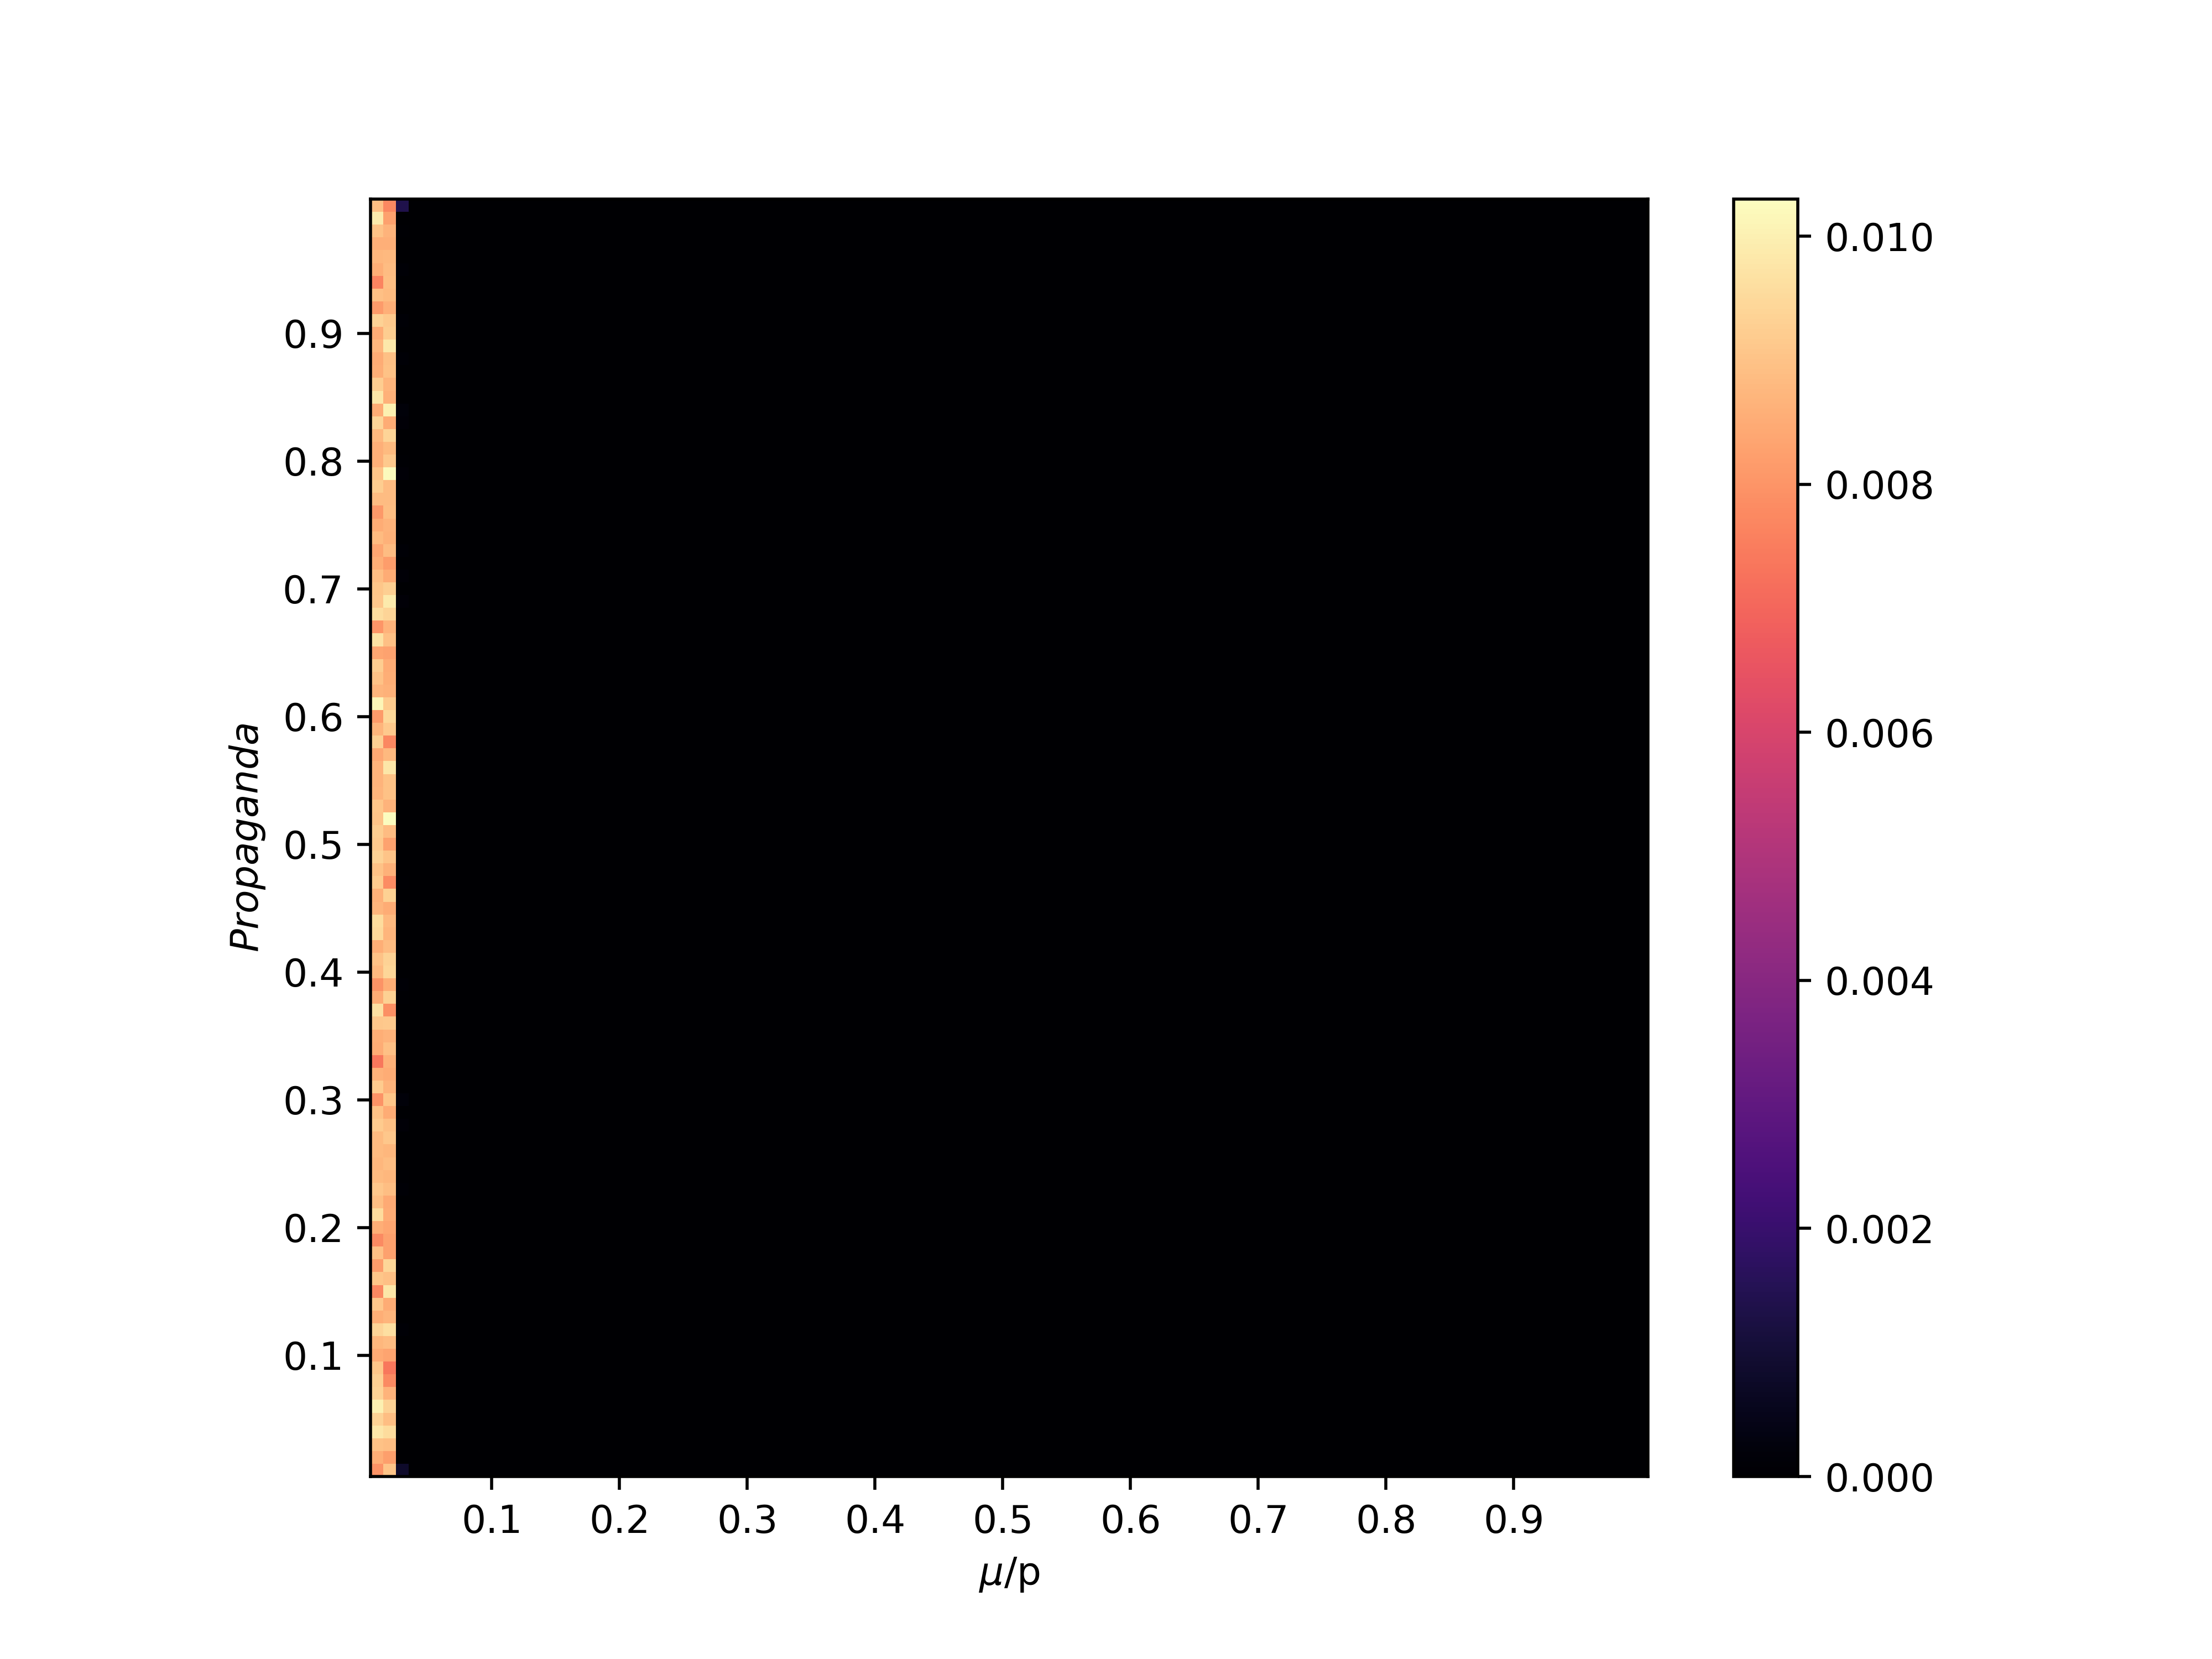
\includegraphics[scale = 0.45]{images/sigma_prop_vs_mu_n1000_p100_i100.png}
    \caption{Heat map of $\sigma$ in function of normalized tolerance $\mu/p$ and the mass media state for fixed value of intensity $\beta = 1.0$.}
    \label{fig:sigma_prop_vs_tolerance_i10}
\end{figure}
\begin{figure}
    \centering
    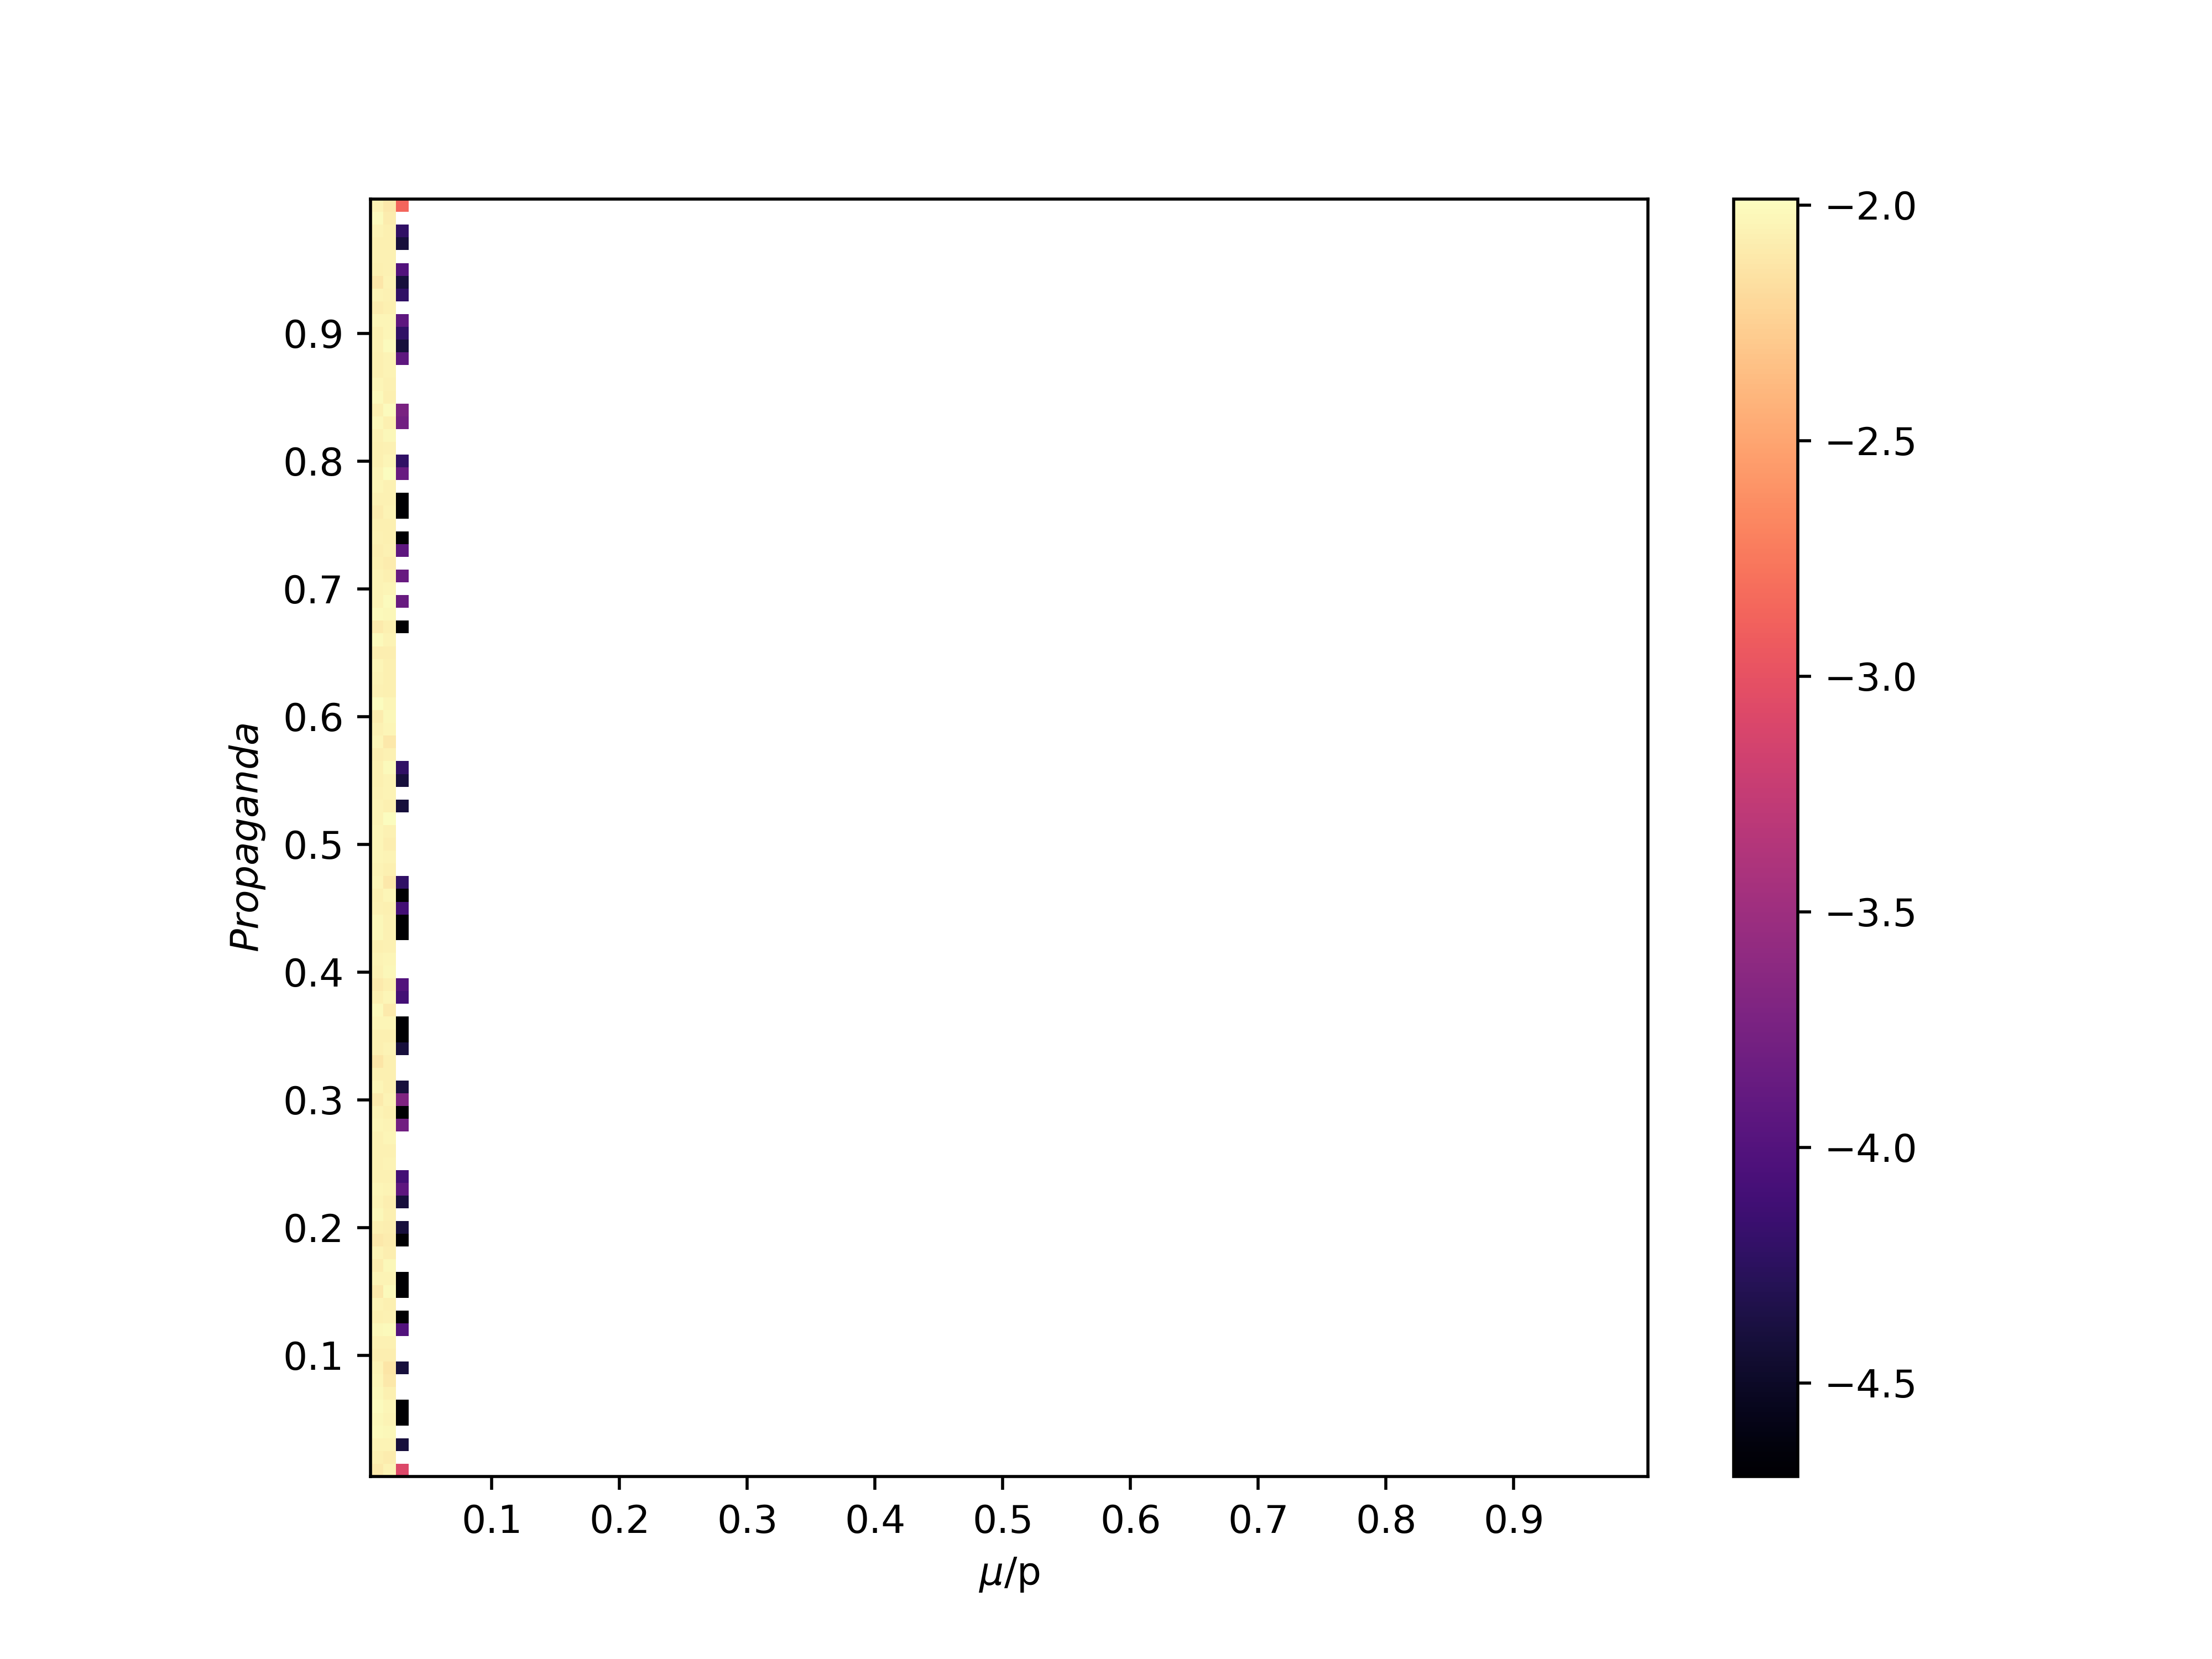
\includegraphics[scale = 0.45]{images/logsigma_prop_vs_mu_n1000_p100_i100.png}
    \caption{Heat map of \log($\sigma$) in function of normalized tolerance $\mu/p$ and the mass media state for fixed value of intensity $\beta = 1.0$.}
    \label{fig:logsigma_prop_vs_tolerance_i10}
\end{figure}



\section{Conclusions}




\printbibliography{}

\end{document}
%
% ****** End of file apssamp.tex ******
